\documentclass[../main]{subfiles}
\begin{document}

\section{Documentazione}
Riguardo alla documentazione, che corrisponde a un \g{processo} di \g{progetto} nello sviluppo di un \g{prodotto software}, vanno poste tre domande:
\begin{itemize}
    \item Perché documentare?
    \item Cosa documentare?
    \item Come documentare?
\end{itemize}
\subsection{Perche documentare?}
Da un punto di vista altruistico, si può dire che la documentazione è necessaria per il mantenimento del software. Dal punto di vista del fornitore, è possibile che, riprendendo in mano il codice sorgente di un software dopo tanto tempo che non vi ci si lavora, esso non venga compreso se non correttamente documentato. Dal punto di vista del committente invece, potrebbe essere di difficile comprensione un software senza l'utilizzo di un manuale utente.\newline
Da un punto di vista meno altruistico, quasi egoistico (un egoismo finalizzato alla collaborazione), la documentazione risulta necessaria affinché si possa tener traccia dell'avanzamento di un \g{progetto} lungo tutti i suoi \g{processi}, verificando che vengano raggiunti gli obiettivi di qualità dichiarati.\newline
La necessità di tracciare è ovvia: un \g{progetto} svolto con professionalità non può che essere collaborativo e quindi tutti coloro che collaborano devono sapere cosa c'è da fare.
\subsection{Cosa documentare?}
Per ogni attività di progetto esiste un documento e questi documenti sono vivi: sono costantemente aggiornati (a meno che non raggiungano una versione stabile che non necessita più di modifiche) e vanno consultati spesso.
Alcuni documenti da redigere sono:
\begin{itemize}
    \item Gestione di \g{progetto}, ovvero come si intende organizzare in \g{processi} l'intero \g{prodotto}, la definizione del \g{way of working}, i ruoli, le responsabilità, la pianificazione e le risorse;
    \item Amministrazione di progetto, ovvero la gestione della \g{qualità} (tra cui il \g{piano di qualità}), quindi la verifica e la validazione, e la gestione della configurazione;
    \item Analisi dei requisiti, ovvero i requisiti da soddisfare nella realizzazione del \g{prodotto software} affinché il committente soprattutto, ma anche il fornitore, siano soddisfatti;
    \item Progettazione, come si intende implementare ciò che è stabilito nel documento di analisi dei requisiti;
\end{itemize}
Un buon modo di procedere è seguire il così detto \textit{Modello a V}:
\begin{figure}[h]
    \begin{center}
        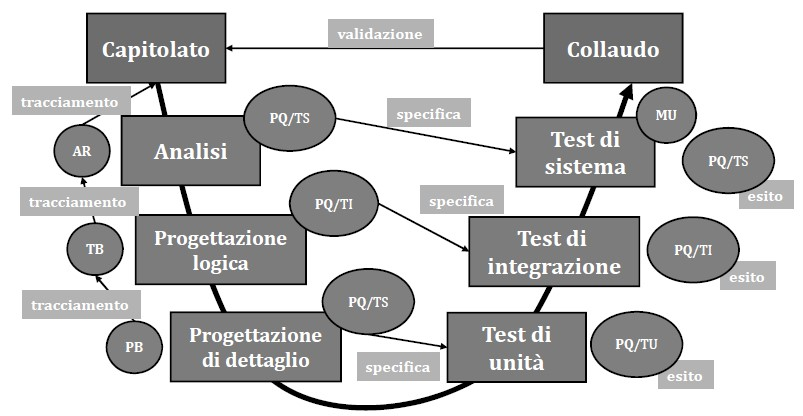
\includegraphics[scale=0.8]{immagini/vmodel.jpg}
    \end{center}
\end{figure}
\subsection{Come documentare?}
Un primo aspetto riguarda la scrittura, in quanto i documenti sono testi scritti. Può essere utile utilizzare il seguente come vademecum:
\begin{itemize}
    \item Utilizzo di verbi in forma attiva, poiché quelli passivi potrebbero confondere il vero attore dell'azione;
    \item Titolazione e numerazione di sezioni e sottosezioni, per una maggior facilità di ricerca e di navigazione all'interno e fra i documenti;
    \item Correttezza grammaticale e tipografica (serve dirlo?);
    \item Precisione terminologica, anche attraverso la redazione di un glossario, come per questo fantastico riassunto. Non è possibile avere terminologia ambigua, è troppo rischiosa;
    \item Evitare la verbosità, preferendo frasi brevi e su di un unico argomento (che il tempo è denaro, e il denaro non c'è, ma nemmeno il tempo);
    \item Preferire le liste e gli elenchi puntati a narrazioni;
    \item Argomenti complessi richiedono spiegazioni più spiegazioni da più punti di vista. Spiegazioni accurate possibilmente, e non semplificate.
\end{itemize}
Per la scrittura della documentazione è necessario utilizzare strumenti che permettano la scrittura collaborativa. Un esempio famoso è Google Docs, ma può essere anche utilizzato \LaTeX{} versionando i \textit{sorgenti} su di un repository. I \textit{sorgenti} non a caso è \textit{plurale}, infatti sarebbe bene che il documento fosse scritto a moduli (o diviso in sezioni a cui corrispondo più file), come se fosse un software.\newline
Deve essere poi decisa la struttura del documento, che deve essere chiara a tutti i destinatari e lettori della documentazione, i destinatari e la storia (ossia il registro delle modifiche, con redattori, date di modifiche e verificatori).\newline
Un altro aspetto importante è il tracciamento. Si tratta di tracciare tutto ciò che viene fatto, attraverso delle matrici di tracciabilità.\newline
Il tracciamento può essere visto:
\begin{itemize}
    \item In avanti (per fini di completezza), il che significa che ad ogni input ad una fase deve corrispondere successivamente un'output;
    \item All'indietro (per necessità), e quindi ad ogni output deve corrispondere un input.
\end{itemize}
Ovvero ad ogni azione segue un'altra.
In un \g{progetto} software il tracciamento deve essere fatto seguendo il \textit{Modello a V}, quindi:
\begin{itemize}
    \item Capitolato $\leftrightarrow$ Analisi dei requisiti;
    \item Analisi dei requisiti $\leftrightarrow$ Componenti architetturali (della Technology Baseline);
    \item Componenti architetturali (della Technology Baseline) $\leftrightarrow$ Moduli software (della Product Baseline);
    \item Moduli software (della Product Baseline) $\leftrightarrow$ Test di unità;
    \item Componenti architetturali (della Technology Baseline) $\leftrightarrow$ Test di integrazione;
    \item Analisi dei requisiti $\leftrightarrow$ Test di sistema;
    \item Capitolato $\leftrightarrow$ Test di accettazione;
\end{itemize}
\end{document}